\qrchapter{https://forgottenpillar.com/rsc/en-fp-chapter2}{The Fundamental Principles}


\qrchapter{https://forgottenpillar.com/rsc/en-fp-chapter2}{Kanuni za Msingi}


The real issue according to chapter ten of the Special Testimonies is diverting from the foundation of our faith, which was established at the beginning of our work.


Suala halisi kwa mujibu wa sura ya kumi ya Shuhuda Maalum ni kuhusu kuachana na msingi wa imani yetu, ambao ulianzishwa mwanzoni mwa kazi yetu.


\egw{\textbf{This foundation was built by the Masterworker}, and \underline{will} stand storm and tempest. Will they permit this man to \textbf{present doctrines that deny the past experience} of the people of God? The time has come to take decided action.}[SpTB02 54.2; 1904][https://egwwritings.org/read?panels=p417.276]


\egw{\textbf{Msingi huu ulijengwa na Mfanyakazi Mkuu}, na \underline{utasimama} dhoruba na tufani. Je, watamruhusu mtu huyu \textbf{kuwasilisha mafundisho yanayopinga uzoefu wa awali} wa watu wa Mungu? Wakati umefika wa kuchukua hatua maalum.}[SpTB02 54.2; 1904][https://egwwritings.org/read?panels=p417.276]


Kellogg presented doctrines that deny the past experience. In another place, she wrote about Kellogg:


Kellogg aliwasilisha mafundisho ambayo yanakataa uzoefu uliopita. Katika sehemu nyingine, aliandika kuhusu Kellogg:


\egw{I am much worried about Dr. Kellogg. In many respects, his course is not pleasing to the Lord. It seems to be \textbf{so easy for him to drift away from \underline{foundation principles}}. He is in great danger \textbf{of not holding the beginning of his confidence} steadfast unto the end.}[Lt138-1902.5; 1902][https://egwwritings.org/read?panels=p9219.11]


\egw{Nina wasiwasi sana kuhusu Dkt. Kellogg. Katika mambo mengi, kozi yake haipendezi Bwana. Inaonekana kuwa \textbf{ni rahisi sana kwake kuachana na \underline{kanuni za msingi}}. Yuko katika hatari kubwa \textbf{ya kutoshikilia imani yake thabiti ya mwanzo} hadi mwisho.}[Lt138-1902.5; 1902][https://egwwritings.org/read?panels=p9219.11]


The problem was the departing from the foundation principles—but not all people recognized that. Especially the key and prominent people in the work; they forgot the way the Lord led them and His teaching in the past.


Tatizo lilikuwa ni kujitenga na kanuni za msingi—lakini si watu wote walitambua hiyo. Hasa watu wakuu na maarufu katika kazi; walisahau njia ya Bwana alivyowaongoza na mafundisho Yake ya awali.


\egw{I have been hoping that there would be a thorough reformation, and that \textbf{the principles} for which we fought \textbf{in the early days}, and which were brought out in the power of the Holy Spirit, \textbf{would be maintained}.}[SpTB02 56.3; 1904][https://egwwritings.org/read?panels=p417.287]


\egw{Nimekuwa nikitumaini kwamba kungekuwa na mageuzi ya kina, na kwamba \textbf{kanuni} ambazo tulizipigania \textbf{siku za kwanza}, na ambazo zilitolewa katika nguvu ya Roho Mtakatifu, \textbf{zingedumishwa}.}[SpTB02 56.3; 1904][https://egwwritings.org/read?panels=p417.287]


What were the principles that we fought for in the early days? What was this foundation of our faith?


Ni kanuni gani tulizopigania katika siku za kwanza? Ni upi msingi wa imani yetu?


\egw{As a people, we are to \textbf{stand firm on the platform of eternal truth} that has withstood test and trial. We are to \textbf{hold to the sure pillars of our faith}. \textbf{The \underline{principles of truth}} that God has revealed to us \textbf{are our only true foundation}. They have made us what we are...}[SpTB02 51.2; 1904][https://egwwritings.org/read?panels=p417.261]


\egw{Kama watu, tunapaswa \textbf{kusimama kidete kwenye jukwaa la ukweli wa milele} ambao umestahimili mtihani na majaribio. Tunapaswa \textbf{kushikilia nguzo za hakika za imani yetu}. \textbf{\underline{Kanuni za ukweli}} ambazo Mungu ametufunulia \textbf{ndio msingi wetu wa kweli}. Zimetufanya tulivyo...}[SpTB02 51.2; 1904][https://egwwritings.org/read?panels=p417.261]


The \egwinline{principles of truth} that God has revealed \egwinline{is our only true foundation}. She is calling these principles the platform of eternal truth. She refers to these principles as the \egwinline{sure pillars of our faith}[SpTB02 51.2; 1904][https://egwwritings.org/read?panels=p417.261].


\egwinline{Kanuni za ukweli} ambazo Mungu amefunua \egwinline{ndio msingi wetu wa kweli}. Anaziita kanuni hizi jukwaa la ukweli wa milele. Anarejelea kanuni hizi kama \egwinline{nguzo za imani yetu}[SpTB02 51.2; 1904][https://egwwritings.org/read?panels=p417.261].


She recalls the past experience of our pioneers, like James White, Joseph Bates, Elder Edson, father Pierce, how God worked on them until \egwinline{point by point}, \egwinline{all \textbf{the principal points of our faith} were made clear}. She recalled how \egwinline{this foundation was built by the Masterworker,} and assures that it \egwinline{will stand storm and tempest}. In conclusion, she strongly affirms the will of God for us regarding these principles. God \egwinline{calls upon us to \textbf{hold firmly}, with the grip of faith, \textbf{to the fundamental principles that are based upon unquestionable authority}}.


Anakumbuka uzoefu uliopita wa wazee wetu, kama James White, Joseph Bates, Mzee Edson, baba Pierce, jinsi Mungu alivyofanya kazi nao mpaka \egwinline{pointi kwa pointi}, \egwinline{\textbf{pointi kuu za imani yetu} zikawekwa wazi}. Alikumbuka jinsi \egwinline{msingi huu ulijengwa na Mjenzi mkuu,} na kuhakikishia kwamba \egwinline{utasimama dhoruba na tufani}. Kwa kumalizia, anatuthibitishia mapenzi ya Mungu kwetu kuhusu kanuni hizi. Mungu \egwinline{anatuita \textbf{tushike kwa imara}, kwa mshiko wa imani, \textbf{kanuni za msingi ambazo mamlaka wake ni usio na shaka}}.


We see several different expressions that Sister White used for the foundation of our faith: “\textit{the platform of eternal truth},” “\textit{pillars of our faith},” “\textit{principles of truth},” “\textit{principal points},” “\textit{waymarks},” “\textit{foundation principles},” and “\textit{fundamental principles}”. These expressions denote the same thing—the foundation of our faith. When we hear these expressions today, somehow they don’t convey any concrete information. But for Seventh-day Adventists in her time, this was very clear and a definite point. All of these terms are referring to the public synopsis of Seventh-day Adventist’s faith called the \emcap{Fundamental Principles}, further explained below.


Tunaona semi kadhaa ambazo Dada White alitumia kwa msingi wa imani yetu: “\textit{jukwaa la ukweli wa milele},” “\textit{nguzo za imani yetu},” “\textit{kanuni za ukweli},” “\textit{pointi kuu},” “\textit{alama za njia},” “\textit{kanuni za msingi},” na “\textit{kanuni za kimsingi}”. Semi hizi zinaashiria jambo moja—msingi wa imani yetu. Leo tunaposikia semi hizi, kwa namna fulani hazifikishi habari yoyote thabiti. Lakini kwa Waadventista Wasabato wa siku za Ellen White, semi hizi zilikuwa na maana ya wazi sana. Semi hizi zote zinaashiria muhtasari wa umma wa imani ya Waadventista Wasabato iitwayo \emcap{Kanuni za Msingi}, kama ilivyoelezwa zaidi hapa chini.


God \egwinline{calls upon us to \textbf{hold firmly}, with the grip of faith, to \textbf{the \underline{fundamental principles}} that  are \textbf{based upon unquestionable authority}.} This is a reference to principal features of Seventh-day Adventist faith which God revealed to Adventist pioneers \egwinline{after the passing of the time in 1844,} when a group of keen, noble, and true men \egwinline{searched for the truth as for hidden treasure.} This was \textit{the foundation of our faith}. Our pioneers officially established the Seventh-day Adventist Church in 1863, and they taught these truths which they called “\textit{fundamental principles}.” But often, Seventh-day Adventists were misrepresented publicly. For this reason, in 1872, our pioneers published a document called “\textit{A Declaration of the Fundamental Principles, Taught and Practiced by the Seventh-day Adventists}” in order to publicly, but briefly, declare what \emcap{fundamental principles} Seventh-day Adventists taught and practiced. These \emcap{Fundamental Principles} were regularly printed as a standalone pamphlet, were present in our papers, and were annually printed in Adventist Yearbooks throughout Ellen White's lifetime.\footnote{See \hyperref[appendix:timeline]{Fundamental Principles - Timeline} for more details.} Therefore, when Ellen White referenced the “\textit{fundamental principles},” this was not a vague or opaque statement, since the Seventh-day Adventist church had officially and publicly declared what these \emcap{fundamental principles} were. In the preface of this document, we read the purpose behind this document.


Mungu \egwinline{anatuita \textbf{kushika kwa uthabiti}, kwa mshiko wa imani, \textbf{\underline{kanuni za msingi}} ambazo zinatokana na \textbf{mamlaka isiyotiliwa shaka}.} Hii ni rejeo kwa mambo makuu ya imani ya Waadventista Wasabato ambayo Mungu aliwafunulia wazee wa Waadventista \egwinline{baada ya kupita kwa wakati wa 1844,} wakati kundi la watu wenye bidii, waungwana na wa kweli \egwinline{walitafuta ukweli kama hazina iliyofichwa.} Huu ulikuwa \textit{msingi wa imani yetu}. Wazee wetu walianzisha rasmi Kanisa la Waadventista Wasabato mwaka 1863, na walifundisha kweli hizi walizoziita “\textit{kanuni za msingi}.” Lakini mara nyingi, Waadventista Wasabato waliwasilishwa vibaya hadharani. Kwa sababu hii, mwaka 1872, wazee wetu walichapisha waraka ulioitwa “\textit{A Declaration of the Fundamental Principles, Taught and Practiced by the Seventh-day Adventists}” ili kutangaza hadharani, kwa ufupi, ni \emcap{kanuni za msingi} gani Waadventista Wasabato walifundisha na kutenda. Hizi \emcap{Kanuni za Msingi} zilichapishwa mara kwa mara kama kijitabu, zilikuwepo katika magazeti yetu, na zilichapishwa kila mwaka katika Vitabu vya Mwaka vya Waadventista katika maisha yote ya Ellen White.\footnote{Tazama \hyperref[appendix:timeline]{Kanuni za Msingi - Mstari wa Wakati} kwa maelezo zaidi.} Kwa hiyo, Ellen White aliporejea “\textit{kanuni za msingi},” hii haikuwa kauli isiyoeleweka au isiyowazi, kwani kanisa la Waadventista Wasabato lilikuwa limetangaza rasmi na hadharani ni \emcap{kanuni za msingi} gani. Katika utangulizi wa waraka huu, tunasoma lengo la waraka huu.


\begin{figure}
    \centering
    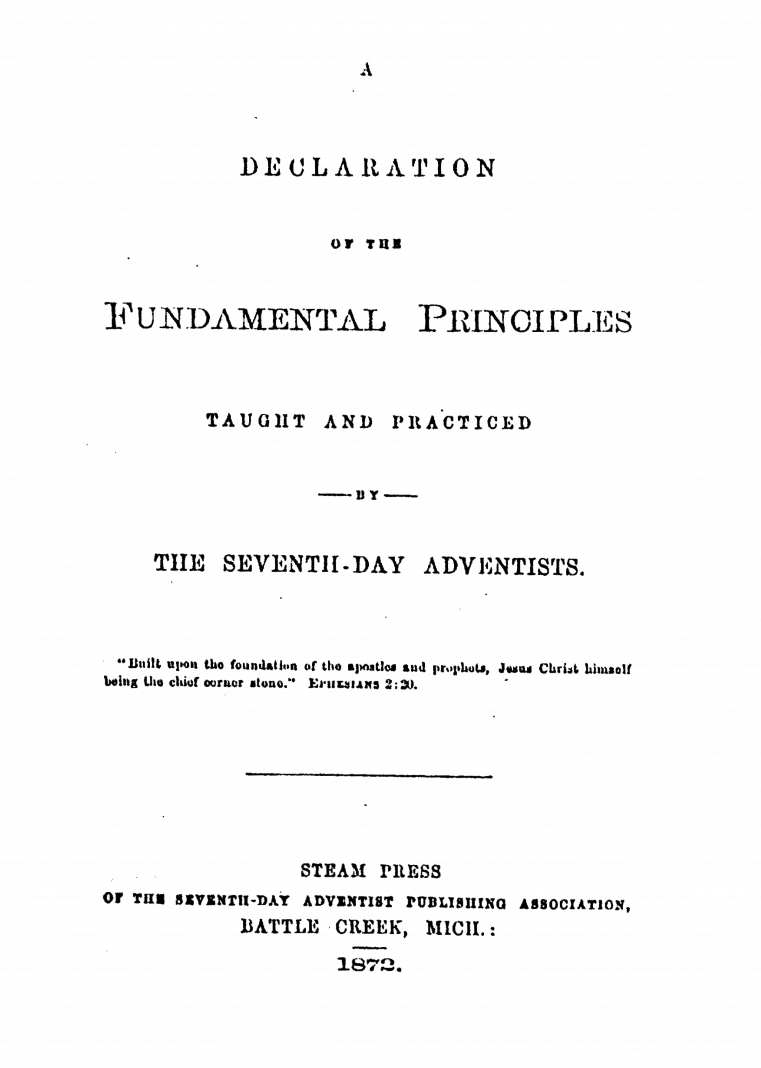
\includegraphics[width=1\linewidth]{images/declaration-of-the-fundamental-principles.PNG}
    \caption*{Scan of the Declaration of the Fundamental Principles, 1872.}
    \label{fig:declaration-of-the-fundamental-principles}
\end{figure}


\begin{figure}
    \centering
    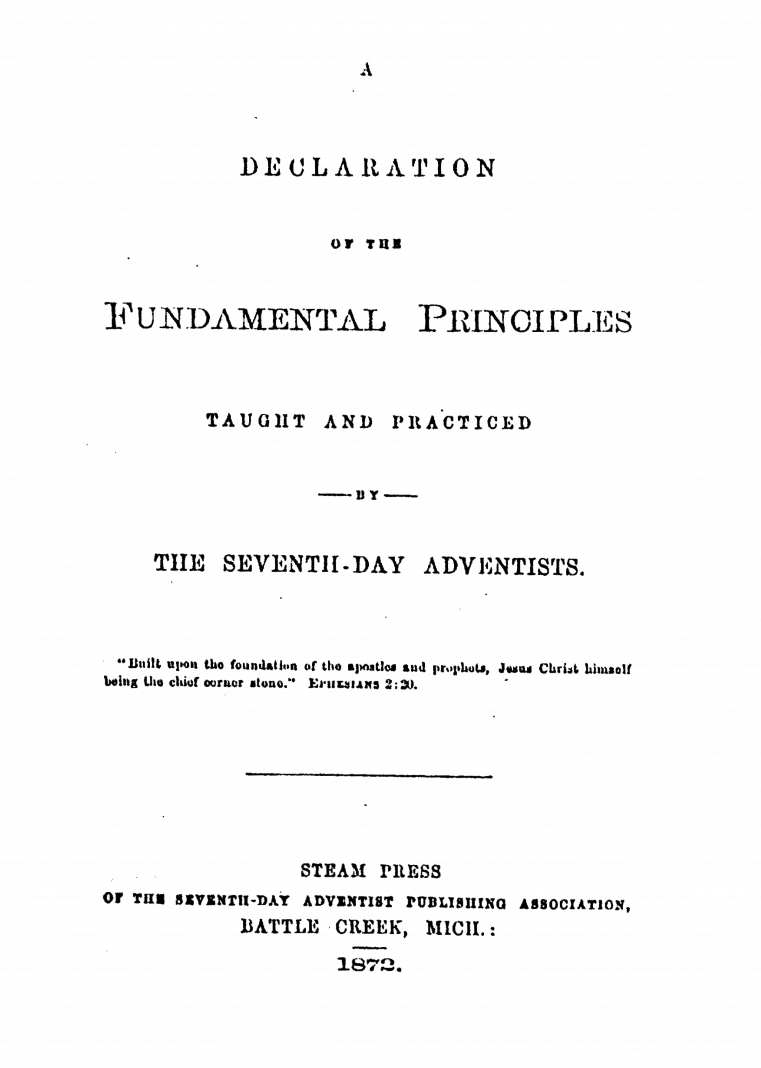
\includegraphics[width=1\linewidth]{images/declaration-of-the-fundamental-principles.PNG}
    \caption*{Picha ya Tamko la Kanuni za Msingi, 1872.}
    \label{fig:declaration-of-the-fundamental-principles}
\end{figure}


\others{In presenting to the \textbf{public} this \textbf{synopsis of our faith}, we wish to have it distinctly understood that \textbf{we have no articles of faith, creed, or discipline, }\textbf{\underline{aside from the Bible}}. We \textbf{do not} put forth this as \textbf{having any authority with our people}, \textbf{nor is it designed to secure uniformity among them}, \textbf{as a system of faith}, \textbf{but is a brief statement of \underline{what is, and has been, with great unanimity, held by them}}. We often find it necessary to meet inquiries on this subject, and sometimes to correct false statements circulated against us, and to remove erroneous impressions which have obtained with those who have not had an opportunity to become acquainted with our faith and practice. Our only object is to meet this necessity.}


\others{Katika kuwasilisha kwa \textbf{umma} muhtasari huu wa imani yetu, tunataka ieleweke kwa uwazi kwamba \textbf{hatuna vifungu vya imani, kanuni za imani, au nidhamu, }\textbf{\underline{kando na Biblia}}. \textbf{Hatuweki} haya kuwa na \textbf{mamlaka yoyote juu ya watu wetu}, \textbf{wala hayakusudiwi kufanya usawa kati yao}, \textbf{kama mfumo wa imani}, \textbf{bali ni taarifa fupi ya \underline{wanayoamini kwa umoja mkubwa}}. Mara nyingi tunaona umuhimu wa kukutana na maswali juu ya mada hii, na wakati mwingine kusahihisha taarifa za uwongo zinazosambazwa dhidi yetu, na kuondoa hisia potofu ambazo wanazo wale ambao hawajapata nafasi ya kufahamiana na imani na utendaji wetu. Lengo letu la pekee ni kukutana na haya.}


\othersnogap{\textbf{As Seventh-day Adventists we desire simply that our position shall be understood}; and we are the more solicitous for this because there are many who call themselves Adventists who hold views with which we can have no sympathy, some of which, we think, are subversive of the plainest and most important principles set forth in the word of God...}[The Fundamental Principles 1872, p. 3.1][https://egwwritings.org/read?panels=p928.8]


\othersnogap{\textbf{Kama Waadventista Wasabato tunatamani tu kwamba msimamo wetu utaeleweka}; na tunatamani sana hili kwa sababu wapo wengi wanaojiita Waadventista bali wanashikilia maoni ambayo hatuwezi kuwa na huruma nayo, ambayo baadhi yake, tunafikiri, yanapindua kanuni zilizo wazi na muhimu zaidi zilizowekwa wazi katika neno la Mungu...}[The Fundamental Principles 1872, p. 3.1][https://egwwritings.org/read?panels=p928.8]


This synopsis of faith consisted of 25 points, which represented \others{what is, and has been, with great unanimity, held by} Seventh-day Adventists. These 25 points constituted \egwinline{\textbf{the foundation} that was \textbf{laid at the beginning} of our work \textbf{by prayerful study} of the word and by revelation}. In 1904, Sister White told us that \egwinline{upon \textbf{this foundation} we have been building for \textbf{the past fifty years}.} These are the \egwinline{\textbf{the fundamental principles that are based upon unquestionable authority}}, that God \egwinline{calls upon us to \textbf{hold firmly}, with the grip of faith}. In other words, she repeated, \egwinline{we are to \textbf{hold to the sure pillars of our faith}}.


Muhtasari huu wa imani ulikuwa na mambo 25, ambayo yaliwakilisha \others{wanayoamini kwa umoja mkubwa} Waadventista Wasabato. Mambo haya 25 yalijumuisha \egwinline{\textbf{msingi} ambao \textbf{uliwekwa mwanzoni} mwa kazi yetu \textbf{kwa kujifunza neno kwa maombi} na kwa ufunuo}. Mnamo 1904, Dada White alituambia kwamba \egwinline{juu ya \textbf{msingi huu} tumekuwa tukijenga kwa \textbf{miaka hamsini iliyopita}.} Hizi ndizo \egwinline{\textbf{kanuni za kimsingi ambazo msingi wake ni mamlaka isiyotiliwa shaka}}, kwamba Mungu \egwinline{anatuita \textbf{tushike kwa uthabiti}, pamoja na mshiko wa imani}. Kwa maneno mengine, alirudia, \egwinline{tunapaswa \textbf{kushikilia nguzo za hakika za imani yetu}}.


In 1904, Sister White wrote about\egwinline{the \textbf{efforts of the enemy to undermine the foundation of our faith}}. She wrote about the movement that would\egwinline{consist in \textbf{giving up} the doctrines which stand as \textbf{the pillars of our faith}}. This reformation, if accepted, would discard\egwinline{\textbf{the principles of truth} that God in His wisdom has given to the remnant church} and\egwinline{\textbf{the fundamental principles} that have sustained the work for the last fifty years \textbf{would be accounted as error}}. This movement started about the time when Dr. John H. Kellogg published the book, “Living Temple”.


Mnamo 1904, Dada White aliandika kuhusu \egwinline{\textbf{juhudi za adui kudhoofisha msingi wa imani yetu}}. Aliandika kuhusu vuguvugu ambalo \egwinline{lingehusisha \textbf{kuacha} mafundisho ambayo yanasimama kama \textbf{nguzo za imani yetu}}. Matengenezo haya yakikubaliwa yangetupilia mbali \egwinline{\textbf{kanuni za ukweli} ambazo Mungu katika hekima yake ametoa kwa kanisa la masalio} na \egwinline{\textbf{kanuni za kimsingi} ambazo zimedumisha kazi hiyo kwa miaka hamsini iliyopita \textbf{zingehesabiwa kuwa makosa}.} Vuguvugu hili lilianza wakati ambapo Dk. John H. Kellogg alichapisha kitabu, “Hekalu Hai”.


\egw{About the time that ‘Living Temple’ was published, there passed before me in the night season, \textbf{representations indicating that some danger was approaching}, and that I must prepare for it by \textbf{writing out the things} God has revealed to me \textbf{regarding \underline{the foundation principles of our faith}}.}[SpTB02 52.3; 1904][https://egwwritings.org/read?panels=p417.267]


\egw{Takriban wakati ambapo ‘Hekalu Hai’ ilichapishwa, ilipita mbele yangu katika msimu wa usiku, \textbf{maono zilizoonyesha kwamba hatari fulani ilikuwa inakaribia}, na hivyo ni lazima nijitayarishe kwa \textbf{kuandika mambo} ambayo Mungu amenifunulia \textbf{kuhusu \underline{kanuni za msingi wa imani yetu}}.}[SpTB02 52.3; 1904][https://egwwritings.org/read?panels=p417.267]


By publishing “Living Temple”, \textbf{foundation principles of our faith} \textbf{would be undermined}\egwinline{through the dissemination of \textbf{seductive theories}} contained therein.


Kwa kuchapisha “Hekalu Hai”, \textbf{kanuni za msingi wa imani yetu} \textbf{zingedhoofishwa} \egwinline{kupitia uenezaji wa \textbf{nadharia potofu}} zilizomo humo.


\egw{I have been instructed by the heavenly messenger that some of the reasoning in the book, ‘Living Temple,’ is unsound and that \textbf{this reasoning would lead astray} the minds of those who are not thoroughly established on \textbf{the foundation principles} of present truth. It introduces that which is naught but speculation in \textbf{regard to \underline{the personality of God and where His presence is}}.}[SpTB02 51.3; 1904][https://egwwritings.org/read?panels=p417.262]


\egw{Nimeagizwa na mjumbe wa mbinguni kwamba baadhi ya hoja katika kitabu, ‘Living Temple,’ hazifai na kwamba \textbf{hoja hizi zitapotosha} akili za wale ambao hawajasimama kikamilifu juu ya \textbf{kanuni za msingi} za ukweli wa sasa. Inatanguliza yale ambayo si chochote bali dhana tu kuhusiana na \textbf{\underline{umbile la Mungu na mahali uwepo Wake upo}}.}[SpTB02 51.3; 1904][https://egwwritings.org/read?panels=p417.262]


Sister White is very particular in pointing out that the reasoning contained in the book Living Temple,\egwinline{\textbf{would lead astray}} from the\egwinline{\textbf{the foundation principles} of present truth}. These reasonings are in\egwinline{\textbf{regard to the personality of God and where His presence is}}.


Dada White anakazia sana kuonyesha kwamba hoja iliyo katika kitabu cha Living Temple,\egwinline{\textbf{zitapotosha}} kutoka kwa\egwinline{\textbf{kanuni za msingi} za ukweli wa sasa}. Hoja hizi ni kuhusiana na\egwinline{\textbf{umbile la Mungu na mahali uwepo Wake upo}}.


As mentioned before, the word ‘\textit{personality’}, in the context of the nineteenth century, is defined as “\textit{the quality or state of being a person}”\footnote{\href{https://www.merriam-webster.com/dictionary/personality}{Merriam-Webster Dictionary}, word ‘\textit{personality}’}. In other words, this term conveys the answer to the question, “\textit{what is it that defines someone to be a person?}”, “\textit{What is the quality or state of someone being a person?}” In the case of the \emcap{personality of God}, the question is, “\textit{Is God a person and what is it that defines Him as being a person? What is the quality or state of God being a person?}”


Kama ilivyoelezwa hapo awali, neno ‘\textit{personality}’, katika muktadha wa karne ya kumi na tisa, inamaanisha “\textit{ubora au hali ya kuwa Nafsi}”\footnote{\href{https://www.merriam-webster.com/dictionary/personality}{Merriam-Webster Dictionary}, neno ‘\textit{personality}’}. Kwa maneno mengine, neno hili huwasilisha jibu kwa swali, “\textit{ni nini kinachofafanua yeyote yule kuwa Nafsi?}”, “\textit{Ni nini ubora au hali ya Nafsi kuwa Nafsi?}” Katika suala la \emcap{umbile la Mungu}, swali ni, “\textit{Je, Mungu ni Nafsi na ni nini kinachomfafanua kuwa Nafsi? Ni nini ubora au hali ya Mungu kuwa Nafsi?}”


The reasoning of Dr. Kellogg regarding these questions expressed in the book Living Temple, is\egwinline{unsound}. The sentiments, in\egwinline{\textbf{regard to the personality of God and where His presence is}},\egwinline{advocated in the book, did not bear the indorsement of God, and that they were \textbf{a snare that the enemy had prepared for the last days}}. As we are living in the last days, we ought to ask ourselves these questions. Likewise, we are to question the biblical validity of the statements in the \emcap{Fundamental Principles} regarding the \emcap{personality of God} and where His presence is. How do the \emcap{Fundamental Principles} define God as being a person, and what do they say regarding God’s presence?


Hoja ya Dkt. Kellogg kuhusu maswali hayo iliyoonyeshwa katika kitabu Living Temple, ni\egwinline{halifu}. Maoni, kuhusu\egwinline{\textbf{umbile la Mungu na mahali uwepo Wake upo}},\egwinline{yanayotetewa katika kitabu, hayana idhini ya Mungu, na ni \textbf{mtego ambao adui alikuwa ametayarisha kwa siku za mwisho}}. Kama tunaishi katika siku za mwisho, tunapaswa kujiuliza maswali haya. Vivyo hivyo, tunapaswa kuhoji uhalali wa kibiblia wa kauli zilizo katika \emcap{Kanuni za Msingi} kuhusu \emcap{umbile la Mungu} na mahali uwepo wake upo. Je, \emcap{Kanuni za Msingi} zinafafanuaje Mungu kuwa Nafsi, na zinasema nini kuhusu uwepo wake?


The first point listed below deals with the \emcap{personality of God} and His presence. The second point gives the context to the first. Please consider a few questions while reading them: Who is referred to as one God? How is God defined as a person or in other words, what is the quality or state of Him being a person? How do these points talk about the presence of God?


Jambo la kwanza lililoorodheshwa hapa chini linahusu \emcap{umbile la Mungu} na uwepo wake. La pili linatoa muktadha wa la kwanza. Tafadhali zingatia maswali haya unapoyasoma: Nani anaashiriwa kuwa Mungu mmoja? Mungu anafafanuliwaje kuwa Nafsi au kwa maneno mengine, ni nini ubora au hali ya Yeye kuwa Nafsi? Je, mambo haya yanazungumziaje uwepo wa Mungu?


\others{“I – That there is \textbf{one God}, \textbf{\underline{a personal, spiritual being}}, \textbf{the creator of all things}, omnipotent, omniscient, and eternal, infinite in wisdom, holiness, justice, goodness, truth, and mercy; unchangeable, and \textbf{\underline{everywhere present by his representative, the Holy Spirit}}. Ps. 139:7.”}


\others{“I – Kwamba kuna \textbf{Mungu mmoja}, \textbf{\underline{nafsi ya kibinafsi, ya kiroho}}, \textbf{Muumba wa vitu vyote}, mwenye uwezo wote, mwenye kujua yote, na wa milele, asiye na kikomo katika hekima, utakatifu, haki, wema, ukweli, na rehema; asiyebadilika, na \textbf{\underline{aliye kila mahali kupitia kwa mwakilishi wake, Roho Mtakatifu}}. Zab. 139:7.”}


\othersnogap{II – That there is \textbf{one Lord Jesus Christ, }\textbf{\underline{the Son of the Eternal Father}}, the one \textbf{\underline{by}}\textbf{ whom God created all things}, and by whom they do consist; …”}[The Fundamental Principles 1889, point no. 1.,2.,.] \footnote{See \hyperref[chap:appendix]{Appendix} for the full list of the Fundamental Principles} \footnote{From 1872 until 1914, the Fundamental Principles remained constant and unchanged, with the exception in 1889, when James Smith added three new points. But during all those years, the points concerning “\textit{the personality of God}” and “\textit{where His presence is}” remained the same. }


\othersnogap{II – Kwamba kuna \textbf{Bwana mmoja Yesu Kristo, }\textbf{\underline{Mwana wa Baba wa Milele}}, ambaye \textbf{\underline{kupitia}}\textbf{ kwake Mungu aliumba vitu vyote}, na kupitia kwake vitu hivyo vinadumu; …“}[The Fundamental Principles 1889, point no. 1.,2.,.] \footnote{Tazama \hyperref[chap:appendix]{Kiambatisho} kwa orodha kamili ya Kanuni za Msingi} \footnote{Kutoka 1872 hadi 1914, Kanuni za Msingi zilisalia thabiti na bila mabadiliko, isipokuwa mwaka 1889, wakati James Smith alipoongeza pointi tatu mpya. Lakini katika miaka yote hiyo, pointi zinazohusiana na “\textit{umbile la Mungu}” na “\textit{mahali uwepo Wake upo}” zilisalia sawa.}


In the time of Ellen White, Seventh-day Adventists believed in one God—a personal, spiritual being, the Creator of all things—and they believed that this God created everything by His Son Jesus Christ. They addressed the Father as one God, and they addressed Christ as the Son of God. The quality or state of God being a person is expressed in the term “\textit{personal, spiritual being}”. Regarding His presence, the \emcap{Fundamental Principles} state that He is everywhere present by His representative, the Holy Spirit. The meaning of these principles requires very special attention. Keeping within the historical context, this will be the subject of our following studies.


Katika wakati wa Ellen White, Waadventista Wasabato waliamini katika Mungu mmoja—nafsi ya kibinafsi, ya kiroho, Muumba wa vitu vyote—na waliamini kwamba Mungu huyu aliumba kila kitu kupitia kwa Mwana wake Yesu Kristo. Walimwita Baba, Mungu mmoja, na walimwita Kristo, Mwana wa Mungu. Ubora au hali ya Mungu kuwa Nafsi inaonyeshwa katika neno “\textit{nafsi ya kibinafsi, ya kiroho}”. Kuhusu uwepo wake, \emcap{Kanuni za Msingi} zinaeleza kuwa yuko kila mahali kupitia kwa mwakilishi wake, Roho Mtakatifu. Maana ya kanuni hizi inahitaji umakini maalum sana. Hii itakuwa mada ya masomo yetu yafuatayo.


\section*{The Test}


\section*{Mtihani}


Most obviously, these \emcap{fundamental principles} do not contain the doctrine of the Trinity! More precisely, the sentiments “\textit{three in one},” or “\textit{one in three}”, in reference to God, are nowhere to be found—which are present in today’s \textit{Fundamental Beliefs}. Only the Father is referred to as “\textit{one God’‘}. But before rushing to swift conclusions, and condemning the doctrine of the Trinity as\egwinline{\textbf{seductive theories,}} which\egwinline{\textbf{undermine the foundation of our faith}}, please bear in mind that Sister White presents a comprehensive list of characteristics that must be fulfilled in order for it to be deemed as such.


Ni wazi kuwa \emcap{kanuni hizi za msingi} hazina fundisho la Utatu! Kwa usahihi zaidi, maoni “\textit{watatu katika mmoja},” au “\textit{mmoja katika watatu}”, kuhusiana na Mungu, hayapatikani popote—ambayo yapo katika \textit{Imani za Msingi} za leo. Baba pekee ndiye anayetajwa kama “\textit{Mungu mmoja}”. Lakini kabla ya kuhitimisha haraka, na kushutumu fundisho la Utatu kama\egwinline{\textbf{nadharia za uwongo,}} ambazo\egwinline{\textbf{zinadhoofisha msingi wa imani yetu}}, tafadhali kumbuka kwamba Dada White aliwasilisha orodha ya kina ya sifa ambazo lazima zitimizwe ili lihesabiwe kuwa hivyo.


If the Trinity doctrine is questionable, then the trinitarian sentiments would need to:
\begin{itemize}
    \item rob the people of God of their past experience
    \item destroy the \emcap{personality of God}
    \item tear down the pillars of our faith or lead astray from the foundation principles
    \item be presented as if Mrs. White supported them
\end{itemize}


Ikiwa fundisho la Utatu linatiliwa shaka, basi maoni ya utatu yangehitaji:
\begin{itemize}
    \item kuwaibia watu wa Mungu uzoefu wao wa zamani
    \item kuharibu \emcap{Umbile la Mungu}
    \item kubomoa nguzo za imani yetu au kupotosha kutoka kwa kanuni za msingi
    \item kuwasilishwa kana kwamba Bi. White aliyaunga mkono
\end{itemize}


It is not our intention to deal with any of Kellogg’s seductive theories, but rather to study the \emcap{personality of God} in its historical background. As we do this, we will face the evidence of Sister White reactively warning the church of these characteristics.


Sio nia yetu kushughulika na nadharia zozote za kupotosha za Kellogg, bali kusoma \emcap{Umbile la Mungu} kwa muktadha wa historia yake. Tunapofanya hivi, tutakabiliana na ushahidi wa Dada White akitahadharisha kanisa kuhusu tabia hizi.


% The Fundamental Prinicples

\begin{titledpoem}
    \stanza{
        The Masterworker built a foundation strong, \\
        To guide God's people as they journey long. \\
        These truths revealed through prayer and earnest toil, \\
        Stand firm on heaven's unquestionable soil.
    }

    \stanza{
        God as one personal and spiritual being, \\
        Present through His Spirit, all-knowing, all-seeing. \\
        Christ as the Son of the Eternal Father, \\
        These pillars of faith we should hold, not bother.
    }

    \stanza{
        When men depart from these principles true, \\
        Undermining foundations through teachings new, \\
        The wisdom of ages they quickly discard, \\
        And God's revealed pathway becomes sadly marred.
    }

    \stanza{
        Hold firmly the truth with unwavering grip, \\
        Let not from these anchors your faith ever slip. \\
        For what God established through pioneers' hands, \\
        Through tempest and storm eternally stands.
    }
\end{titledpoem}


% The Fundamental Prinicples

\begin{titledpoem}
    \stanza{
        The Masterworker built a foundation strong, \\
        To guide God's people as they journey long. \\
        These truths revealed through prayer and earnest toil, \\
        Stand firm on heaven's unquestionable soil.
    }

    \stanza{
        God as one personal and spiritual being, \\
        Present through His Spirit, all-knowing, all-seeing. \\
        Christ as the Son of the Eternal Father, \\
        These pillars of faith we should hold, not bother.
    }

    \stanza{
        When men depart from these principles true, \\
        Undermining foundations through teachings new, \\
        The wisdom of ages they quickly discard, \\
        And God's revealed pathway becomes sadly marred.
    }

    \stanza{
        Hold firmly the truth with unwavering grip, \\
        Let not from these anchors your faith ever slip. \\
        For what God established through pioneers' hands, \\
        Through tempest and storm eternally stands.
    }
\end{titledpoem}
